\documentclass[11pt,a4paper]{article}
\usepackage[dvipsnames]{xcolor}
\usepackage[T1]{fontenc}
\newcommand{\hsh}[1]{{\texttt{\scriptsize #1}}}
\usepackage[utf8]{inputenc}
\usepackage{lmodern,microtype}
\usepackage{amsmath,amssymb,booktabs,graphicx,array,caption,url}
\usepackage[a4paper,margin=2.3cm]{geometry}
\usepackage[colorlinks=true,linkcolor=blue!50!black,urlcolor=blue!50!black,citecolor=blue!50!black]{hyperref}
\captionsetup{font=small,labelfont=bf}
\setlength{\parindent}{0pt}\setlength{\parskip}{4pt}

\usepackage[english]{babel}
\title{\textbf{med6m: a LoRA adapter for Qwen3-8B on medical multiple-choice QA}\\[2pt]\large Sealed-test evidence for checkpoint 443 at LoRA scale 0.5}
\author{Giovanni Del Papa --- independent researcher, Italy\\ \small Project \emph{Lo Scienziato Dilettante GDP}}
\date{2 November 2026\\ \small Version 1.0 --- DOI \href{https://doi.org/10.5281/zenodo.23895100}{10.5281/zenodo.23895100}\\ \small Hugging Face \texttt{odelpa/qwen3-8b-med6m} $\cdot$ GitHub \texttt{usergdp136/qwen3-8b-med6m}}
\begin{document}\maketitle
\begin{abstract}
We release a LoRA adapter (rank 64) for \texttt{unsloth/Qwen3-8B-unsloth-bnb-4bit}, trained with QLoRA on a six-month medical mix (MedMCQA-train, MedQA-train, Italian and English medical Wikipedia) plus 22\% general replay. On a \emph{sealed, single-use} test of 3\,766 medical multiple-choice items (MedMCQA, MedQA, six MMLU medical subdomains, PubMedQA) the adapter at LoRA scale $s=0.5$ improves accuracy over the base model by $+2.34$ percentage points (pp), 95\% paired-bootstrap CI $[+1.14,+3.53]$, exact McNemar $p=1.4\times10^{-4}$ (306 items only the adapter gets right vs.\ 218 only the base). The gain is concentrated in MedMCQA ($+2.89$ pp) and PubMedQA ($+2.78$ pp); MedQA and MMLU-med are positive but their CIs include zero; the Italian general guard (ARC-it) shows no regression ($+0.74$ pp, CI $[-1.29,+2.76]$). Important limits: the evaluated artefact is checkpoint 443, not the final 886; evaluation is answer-letter log-probability, not free generation; no clinical validity is claimed.
\end{abstract}

\section{Method}
\paragraph{Model and adapter.} Base: Qwen3-8B (Apache-2.0), loaded in 4-bit NF4 (bitsandbytes). The adapter is a LoRA on all attention and MLP projections (\texttt{q,k,v,o,gate,up,down}), rank $r=64$, $\alpha=64$, no dropout. For a frozen weight $W_0$ the adapted weight is
\begin{equation}\label{eq:lora}
W \;=\; W_0 \;+\; s\,\frac{\alpha}{r}\,B A,\qquad A\in\mathbb{R}^{r\times d_{\mathrm{in}}},\; B\in\mathbb{R}^{d_{\mathrm{out}}\times r},
\end{equation}
where $s$ is the inference-time LoRA scale (here $s=0.5$, $\alpha/r=1$): the learned update is applied at half strength.

\paragraph{Training.} Two consecutive QLoRA stages on a Tesla T4: stage \texttt{S1\_v2} (885 steps, lr $5\times10^{-5}$, seed 3407) on the four medical sources only; stage \texttt{S1\_v2r} (planned 886 steps, lr $1.3\times10^{-5}$, warm-up 25, seed 3408, grad.\ accumulation 16, max length 2048), initialised from the last adapter of stage 1 and adding 22\% replay (OASST2, Aya, Dolly, Italian Wikipedia, FineWeb-Edu, FineWeb-2-it) to limit forgetting. The \textbf{published artefact is checkpoint 443 of stage \texttt{S1\_v2r}} (50\% of the stage). About $29.5$M effective target tokens were planned for the second stage (medical 78\%, replay 22\%).

\section{Evaluation protocol}
Every item is scored by the log-probability of the answer letter. With the chat template (thinking disabled) and the prompt truncated to 2048 tokens, the prediction is
\begin{equation}\label{eq:mc}
\hat y \;=\; \arg\max_{\ell\in\mathcal{L}} \; z_\ell ,
\end{equation}
where $z_\ell$ is the next-token logit of letter $\ell$ (with and without leading space) and $\mathcal{L}$ the option letters. Free-form generation is \emph{not} evaluated. Benchmarks: MedMCQA (validation), MedQA-USMLE-4-options (test), six medical MMLU subdomains, PubMedQA (\texttt{pqa\_labeled}, question only, no context), and ARC-Italian (challenge) as general guard. The dev/test split is deterministic: SHA-1 of \texttt{"split|"+ID}, parity of the digest. Training data were decontaminated against dev and test with 10-gram matching. The sealed test was run \emph{once} (marker \texttt{TEST\_USED}, 1 Nov 2026) for the base and for checkpoint 443 at $s\in\{0.5,0.75\}$; the test is therefore consumed and cannot be reused for further selection.

\section{Statistics}
For item $i$ let $b_i,c_i\in\{0,1\}$ be the correctness of base and adapter and $d_i=c_i-b_i\in\{-1,0,1\}$. The reported effect is
\begin{equation}\label{eq:delta}
\Delta_{\mathrm{pp}} \;=\; \frac{100}{n}\sum_{i=1}^{n} d_i \;=\; \frac{100\,(n_{+}-n_{-})}{n},
\end{equation}
with $n_+$ ($n_-$) the items only the adapter (only the base) answers correctly. Confidence intervals are percentile paired bootstraps, implemented as multinomial resampling of the counts,
\begin{equation}\label{eq:boot}
\begin{gathered}
(n_-^*,n_0^*,n_+^*)\sim\mathrm{Mult}\!\big(n;\,\hat p\big),\quad \hat p=\big(\tfrac{n_-}{n},\tfrac{n_0}{n},\tfrac{n_+}{n}\big)\\[3pt] \mathrm{CI}_{95}=\big[q_{0.025},\,q_{0.975}\big]\big\{100\,\tfrac{n_+^*-n_-^*}{n}\big\},
\end{gathered}\end{equation}
with $B=20\,000$ replicates and seed 20261101. The exact two-sided McNemar test on the discordant pairs ($n_-+n_+=m$) is
\begin{equation}\label{eq:mcn}
p \;=\; \min\Big\{1,\; 2\sum_{k=0}^{\min(n_-,n_+)}\binom{m}{k}2^{-m}\Big\}.
\end{equation}
The pool concatenates the four medical benchmarks and weights \emph{items}, not benchmarks. No correction for multiple comparisons is applied; per-benchmark $p$-values are descriptive.

\section{Results on the sealed test}
Table~\ref{tab:main} gives the primary result (scale 0.5); Figure~\ref{fig:forest} shows the differences with CIs for both scales; Figure~\ref{fig:acc} the accuracies and Figure~\ref{fig:disc} the gains and losses per item.
\begin{table}[h]\centering\small
\caption{Sealed test, checkpoint 443, \textbf{scale 0.5} vs.\ base. Accuracy in \%; ``+/$-$'' = items only the adapter / only the base answer correctly. $\Delta$ in percentage points with 95\% bootstrap CI; exact McNemar $p$.}\label{tab:main}
\begin{tabular}{lrrrrcrr}\toprule
Set & $n$ & Base & Adapter & $\Delta$ (pp) & 95\% CI & +/$-$ & McNemar $p$ \\ \midrule
MedMCQA & 2078 & 57.31 & 60.20 & +2.89 & [+1.15, +4.62] & 200/140 & 0.001 \\
MedQA & 646 & 62.85 & 64.40 & +1.55 & [$-$1.55, +4.64] & 57/47 & 0.378 \\
MMLU-med & 538 & 78.25 & 79.00 & +0.74 & [$-$1.67, +3.16] & 25/21 & 0.659 \\
PubMedQA & 504 & 57.94 & 60.71 & +2.78 & [+0.60, +5.16] & 24/10 & 0.024 \\
\midrule
Medical pool (n=3766) & 3766 & 61.34 & 63.67 & +2.34 & [+1.14, +3.53] & 306/218 & $<$0.001 \\
\midrule
ARC-it (guard) & 543 & 88.21 & 88.95 & +0.74 & [$-$1.29, +2.76] & 17/13 & 0.585 \\
\bottomrule\end{tabular}\end{table}

\begin{table}[h]\centering\small
\caption{Same test, scale 0.75 (reported for transparency; both scales were evaluated on the same consumed test).}\label{tab:s075}
\begin{tabular}{lrrrrcrr}\toprule
Set & $n$ & Base & Adapter & $\Delta$ (pp) & 95\% CI & +/$-$ & McNemar $p$ \\ \midrule
MedMCQA & 2078 & 57.31 & 60.97 & +3.66 & [+1.83, +5.49] & 230/154 & $<$0.001 \\
MedQA & 646 & 62.85 & 63.31 & +0.46 & [$-$2.63, +3.72] & 56/53 & 0.848 \\
MMLU-med & 538 & 78.25 & 79.00 & +0.74 & [$-$1.86, +3.35] & 28/24 & 0.678 \\
PubMedQA & 504 & 57.94 & 59.72 & +1.79 & [$-$0.40, +4.17] & 22/13 & 0.175 \\
\midrule
Medical pool (n=3766) & 3766 & 61.34 & 63.78 & +2.44 & [+1.17, +3.69] & 336/244 & $<$0.001 \\
\midrule
ARC-it (guard) & 543 & 88.21 & 88.77 & +0.55 & [$-$1.66, +2.76] & 20/17 & 0.743 \\
\bottomrule\end{tabular}\end{table}

\begin{figure}[h]\centering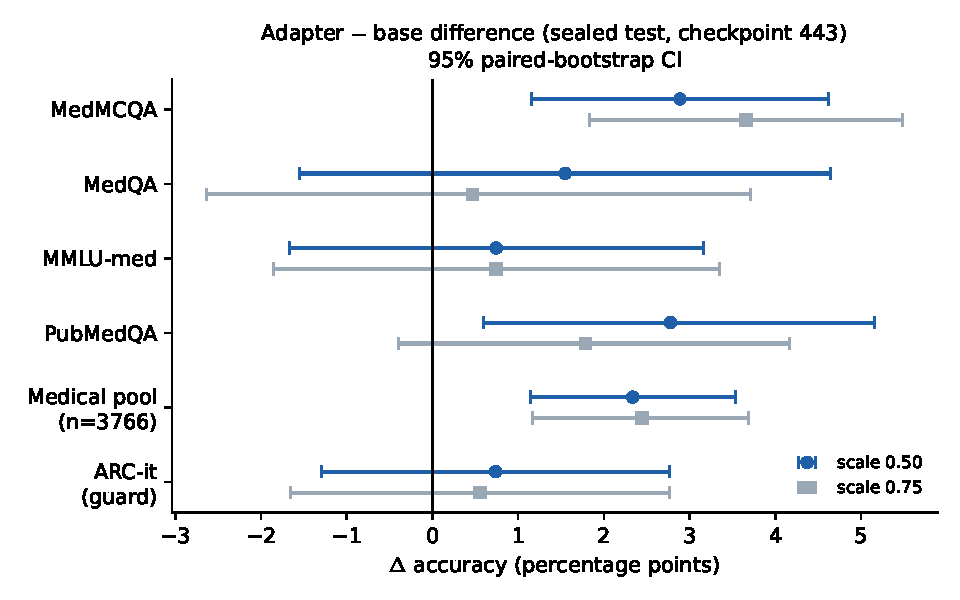
\includegraphics[width=.82\linewidth]{../figures/fig1_forest_en.pdf}\caption{Adapter minus base, sealed test. Points: $\Delta_{\mathrm{pp}}$ (Eq.~\ref{eq:delta}); bars: 95\% CI (Eq.~\ref{eq:boot}).}\label{fig:forest}\end{figure}
\begin{figure}[h]\centering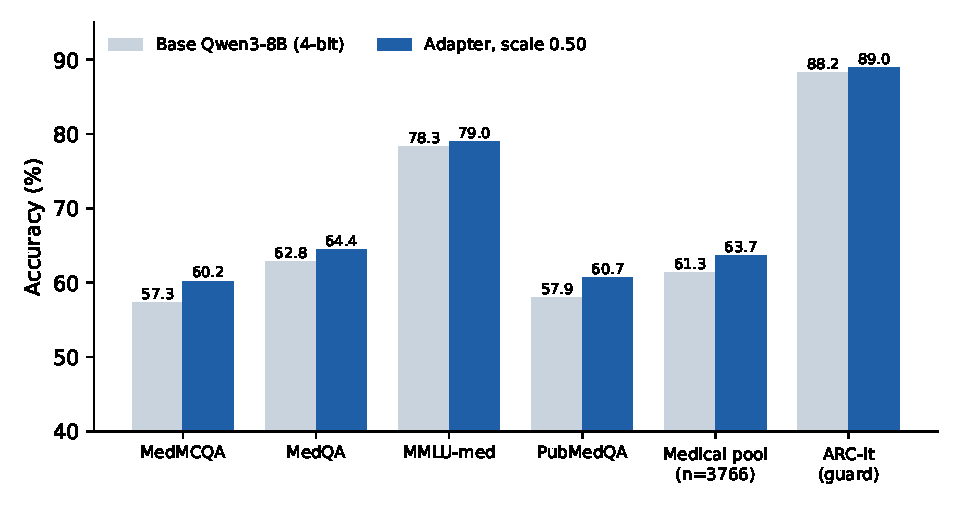
\includegraphics[width=.82\linewidth]{../figures/fig2_acc_en.pdf}\caption{Accuracy of the base and of the adapter (scale 0.5).}\label{fig:acc}\end{figure}
\begin{figure}[h]\centering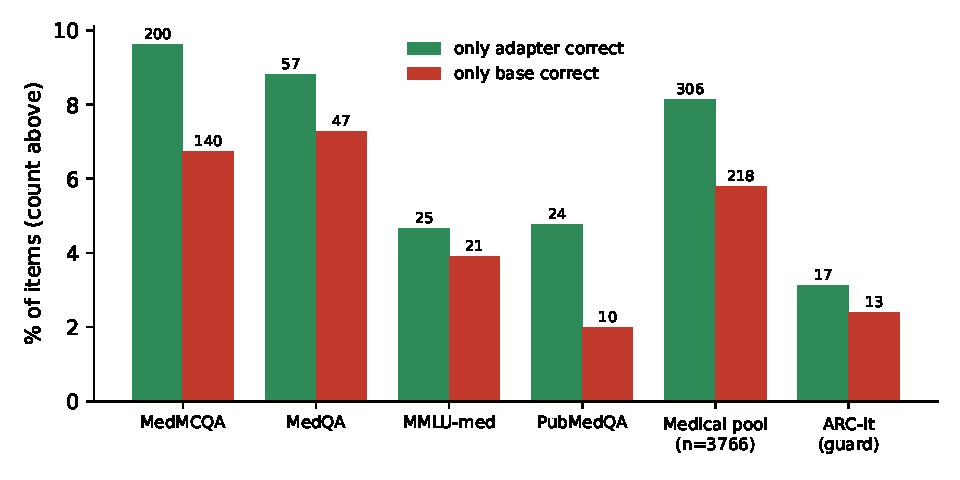
\includegraphics[width=.82\linewidth]{../figures/fig3_disc_en.pdf}\caption{Items only the adapter gets right ($n_+$) versus only the base ($n_-$).}\label{fig:disc}\end{figure}

\paragraph{Reading.} The medical pool improves by $+2.34$ pp (CI excludes 0, $p=1.4\times10^{-4}$). Two benchmarks drive it: MedMCQA (the training mix contains MedMCQA-train, so part of the gain is in-distribution adaptation to the exam format) and PubMedQA. MedQA ($+1.55$) and MMLU-med ($+0.74$) have CIs that include zero: they are \emph{not} confirmed improvements. The guard ARC-it shows no regression on the sealed test. Scales 0.5 and 0.75 are statistically indistinguishable on the pool ($+2.34$ vs.\ $+2.44$ pp).

\section{Final checkpoint 886 on dev (not independent)}
The final checkpoint was evaluated on the dev split only, which guided training decisions (gate, scale). It is therefore \emph{not} an independent confirmation and is not the published artefact.
\begin{table}[h]\centering\small
\caption{DEV split, final checkpoint 886 at scale 1.0 vs.\ base (pool $n=3779$).}
\begin{tabular}{lrrrrcr}\toprule Set & $n$ & Base & Final & $\Delta$ (pp) & 95\% CI & +/$-$ \\ \midrule
MedMCQA & 2105 & 56.25 & 59.48 & +3.23 & [+1.38, +5.08] & 238/170 \\
MedQA & 627 & 62.04 & 65.87 & +3.83 & [+0.48, +7.18] & 70/46 \\
MMLU-med & 551 & 77.13 & 76.41 & $-$0.73 & [$-$3.63, +2.18] & 30/34 \\
PubMedQA & 496 & 53.83 & 55.44 & +1.61 & [$-$0.81, +4.23] & 25/17 \\
Medical pool  & 3779 & 59.94 & 62.48 & +2.54 & [+1.22, +3.84] & 363/267 \\
ARC-it (guard) & 589 & 86.42 & 84.55 & $-$1.87 & [$-$4.07, +0.34] & 18/29 \\
\bottomrule\end{tabular}\end{table}
\begin{figure}[h]\centering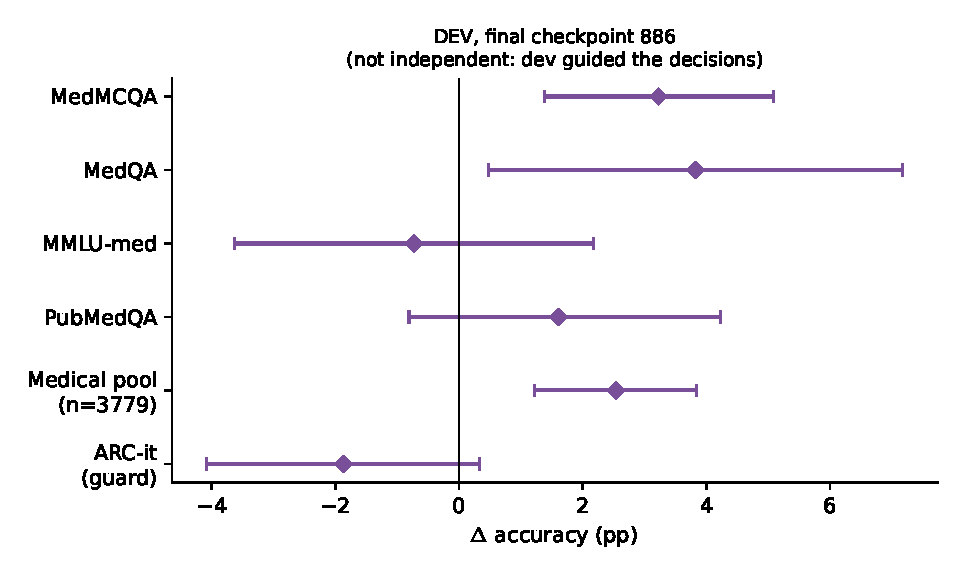
\includegraphics[width=.78\linewidth]{../figures/fig4_dev886_en.pdf}\caption{Dev differences for the final checkpoint 886.}\end{figure}
On dev the final checkpoint gains $+2.54$ pp on the medical pool but loses $-0.73$ pp on MMLU-med and $-1.87$ pp on ARC-it (CIs include 0). The historical gate (two standard errors) accepted it; a stricter criterion (margin $-0.5$ pp, ARC-it floor 85.42\%) would reject it. The gate criterion was revised on 31 Oct 2026 and the 50\% checkpoint was re-rated post hoc. For these reasons we publish checkpoint 443 (which was tested on the sealed set) and \emph{not} the final one.

\section{Limitations and risks}
\begin{itemize}
\item \textbf{Checkpoint vs.\ final.} Evidence concerns checkpoint 443; nothing is claimed for 886.
\item \textbf{Post-selection.} Two scales were evaluated on the same consumed test; scale 0.5 was preferred from dev criteria (smaller ARC-it change, larger PubMedQA gain), but a pre-registered choice does not exist.
\item \textbf{No multiplicity correction}; benchmark-level CIs are descriptive. MedQA and MMLU-med are not significant.
\item \textbf{Task type.} Multiple-choice letter log-probability only; no free-text answers, no safety evaluation, no clinical validation. \emph{Do not use for medical advice.}
\item \textbf{General capability checks pending:} GSM8K and IFEval on checkpoint 443 have \emph{not} yet been run; only the Italian ARC guard is reported.
\item \textbf{Provenance.} MedMCQA-train is declared Apache-2.0 but its exam-question provenance is not independently verified; dataset/model revisions were not pinned at training time (we report the cached revisions available on the training machine, Appendix~A).
\item \textbf{Network audit.} A static review of the training/evaluation code found no non-Hugging-Face endpoints and \texttt{report\_to='none'}; a dynamic (traffic) audit was not performed retroactively (Appendix~B).
\end{itemize}

\section{Licences and attribution}
Base model: Qwen3-8B, Apache-2.0 (\copyright{} Qwen Team / Alibaba Cloud; 4-bit repack by Unsloth). Training sources and licences: MedMCQA-train (Apache-2.0, declared), MedQA-train (MIT, via the \texttt{openlifescienceai/medqa} train split), Wikipedia IT/EN (CC BY-SA 3.0 / GFDL), Dolly-15k (CC BY-SA 3.0), OASST2 and Aya (Apache-2.0), FineWeb-Edu and FineWeb-2 (ODC-By 1.0). All are licences that permit commercial use; none is non-commercial. Because several sources are share-alike, the adapter, the article and the figures are released under \textbf{CC BY-SA 4.0} and the code under Apache-2.0; attribution is in \texttt{ATTRIBUTION.md}. Whether share-alike legally propagates to model weights is unsettled; we apply it conservatively.

\section{Reproducibility}
\texttt{code/recompute.py} recomputes every number in the tables from the paired counts (CPU, NumPy, no network); \texttt{code/make\_figures.py} regenerates the figures. The Codex-assisted audit and our recomputation agree to the second decimal (pool $+2.3367$, CI $[1.1418,3.5316]$). Training and evaluation scripts are provided for inspection; they need the original environment (Unsloth 2026.10.7, Transformers 5.17.0, PEFT 0.21.2, TRL 1.15.0, bitsandbytes 0.50.2, PyTorch 2.11.0+cu128).

\sloppy
\appendix
\section{Pinned artefacts}
\begin{table}[h]\centering\footnotesize
\begin{tabular}{p{5.6cm}p{9.9cm}}\toprule Artefact & SHA-256 / revision \\ \midrule
\hsh{adapter\_model.safetensors} & \hsh{0dfdebe51f325a0d0e1cc5851193a03c4d6aef898ba3b3a595145ab508c4a5bf} \\
\texttt{adapter\_config.json} & \hsh{dcabc2e1d6661d1ad5a18f475a7fd08c875e8cba8664ffbea95bff32d0ce6943} \\
\texttt{tokenizer.json} & \hsh{476870a1f2fb6f6a2759a6ede2383bf9d5d738f17844563b65c91965b722ae09} \\
Base \hsh{unsloth/Qwen3-8B-unsloth-bnb-4bit} & revision \hsh{62efd7f9d748e394734a7adae2adf96e13a2abc8} (cached 24 Oct 2026) \\
\texttt{openlifescienceai/medmcqa} & \hsh{91c6572c454088bf71b679ad90aa8dffcd0d5868} \\
\texttt{GBaker/MedQA-USMLE-4-options} & \hsh{0fb93dd23a7339b6dcd27e241cb9b5eca62d4d18} \\
\texttt{cais/mmlu} & \hsh{c30699e8356da336a370243923dbaf21066bb9fe} \\
\texttt{qiaojin/PubMedQA} & \hsh{9001f2853fb87cab8d220904e0de81ac6973b318} \\
\texttt{sapienzanlp/arc\_italian} & \hsh{1860d09fba59b9b2576335ab472346f63c1becc8} \\
\texttt{wikimedia/wikipedia} & \hsh{b04c8d1ceb2f5cd4588862100d08de323dccfbaa} \\
\bottomrule\end{tabular}\end{table}
\section{Network audit note}
Scope: the med6m code (\texttt{build\_s1v2r.py}, \texttt{train\_stage\_r.py}, \texttt{eval\_mc.py}, \texttt{s0\_data.py}, \texttt{s0b\_data.py}). Finding: network access is limited to Hugging Face datasets/hub downloads for data preparation; \texttt{report\_to='none'} (no W\&B or other trackers); training and scoring read local JSONL files. \texttt{pmc.py} (Europe PMC S3) belongs to the data-preparation helpers and is not part of training/evaluation. Not verified: environment flags (\texttt{HF\_HUB\_OFFLINE}, \texttt{UNSLOTH\_DISABLE\_STATISTICS}) were not found in the launch scripts, so library telemetry cannot be excluded; a clean offline re-run with traffic capture is recommended.
\begin{thebibliography}{9}
\bibitem{qlora} T.~Dettmers et al., \emph{QLoRA: Efficient Finetuning of Quantized LLMs}, 2023. \url{https://arxiv.org/abs/2305.14314}
\bibitem{lora} E.~Hu et al., \emph{LoRA: Low-Rank Adaptation of Large Language Models}, 2021. \url{https://arxiv.org/abs/2106.09685}
\bibitem{qwen3} Qwen Team, \emph{Qwen3 Technical Report}, 2025. \url{https://arxiv.org/abs/2505.09388}
\bibitem{medmcqa} A.~Pal et al., \emph{MedMCQA}, CHIL 2022. \url{https://arxiv.org/abs/2203.14371}
\bibitem{medqa} D.~Jin et al., \emph{What disease does this patient have? (MedQA)}, 2020. \url{https://arxiv.org/abs/2009.13081}
\bibitem{pubmedqa} Q.~Jin et al., \emph{PubMedQA}, EMNLP 2019. \url{https://arxiv.org/abs/1909.06146}
\bibitem{mmlu} D.~Hendrycks et al., \emph{Measuring Massive Multitask Language Understanding}, ICLR 2021. \url{https://arxiv.org/abs/2009.03300}
\end{thebibliography}
\end{document}
